\chapter{Gas e Gas ideali}

\section{Definizioni e legge dei gas perfetti}
\begin{definition}[Mole]
Una \textbf{mole di una sostanza} corrisponde a $6.02\cdot 10^{23}$ particelle di quella sostanza. La costante \`e detta \textbf{numero di Avogadro} e la indichiamo con $N_a$. 
\end{definition}

\begin{definition}[Densit\`a]
Definiamo la \textbf{denstit\`a} come
\[\rho=\frac mV.\]
\end{definition}
\begin{remark}
Il differenziale della densit\`a \`e
\[d\rho=-\frac m{V^2}dV.\]
\end{remark}

\begin{definition}[Condizioni standard]
Un gas \`e in \textbf{condizioni standard} (\textbf{STP}) se \`e alla temperatura di $0^\circ\mathrm C$ e alla pressione di $1\ \mathrm{atm}=101.3245\ \mathrm{kPa}$.
\end{definition}

\noindent Per i gas ideali valgono le seguenti leggi:
\begin{fact}[Legge di Boyle]
Se $T$ \`e costante
\[V\propto \frac1p\]
\end{fact}
\begin{fact}[Legge di Charles]
Se $p$ \`e costante
\[V\propto (1+\al T)\]
\end{fact}
\begin{fact}[Legge di Gay-Lussac]
Se $V$ \`e costante
\[p\propto T\]
\end{fact}
\begin{fact}[Legge di Avogadro]
Se $p$ e $T$ sono fissate, tutti i gas occupano lo stesso volume se consistono della stessa quantit\`a di materia, in particolare
\[V\propto n.\]
Una mole di gas in condizioni standard occupa un volume di $22.4\ell$ (litri).
\end{fact}

\noindent Combinando le leggi appena citate arriviamo alla \textbf{legge dei Gas perfetti}
\[\boxed{pV=nRT}\]
dove $p$ \`e la pressione, $V$ \`e il volume, $n$ \`e il numero di moli, $T$ \`e la temperatura e $R$ \`e la \textbf{costante fondamentale dei gas} e vale $8.314 \frac{\mathrm{J}}{\mathrm{K}\ \mathrm{mol}}$.

\begin{definition}[Costante di Boltzmann]
Definiamo la \textbf{costante di Boltzmann} $k_b$ in modo tale che 
\[R=N_a k_b.\]
\end{definition}

\section{Coefficiente di espansione volumetrica e compressibilit\`a isoterma}

\begin{proposition}[$\al$ e $\beta_T$ per gas ideali]\label{CoefficienteEspansioneECompressibilitaIsotermaPerGasIdeali}
Se il sistema in esame \`e un gas ideale valgono le seguenti identit\`a:
\[\al=\frac 1T,\qquad \beta_T=\frac 1p.\]
\end{proposition}
\begin{proof}
Segue calcolando:
\begin{align*}
\al=&\frac1V\ppb T{(nRT/p)}p=\frac{nR}{pV}=\frac1T,\\
\beta_T=&-\frac1V\ppb p{(nRT/p)}T=\frac1V nRT\frac1{p^2}=\frac1p.
\end{align*}
\end{proof}

\section{Capacit\`a termica}

\begin{definition}[Coefficiente di Joule]
Definiamo il \textbf{coefficiente di Joule} come
\[\mu_J=\ppb VTU\]
\end{definition}

\begin{fact}[In gas ideale l'energia interna dipende solo dalla temperatura]\label{InGasIdealeUdipendeSoloDaT}
In un gas ideale $U$ dipende solo da $T$.
\end{fact}
\begin{proof}[Esperimento: Espansione libera adiabatica di Joule]
\begin{figure}[!htb]
    \centering
    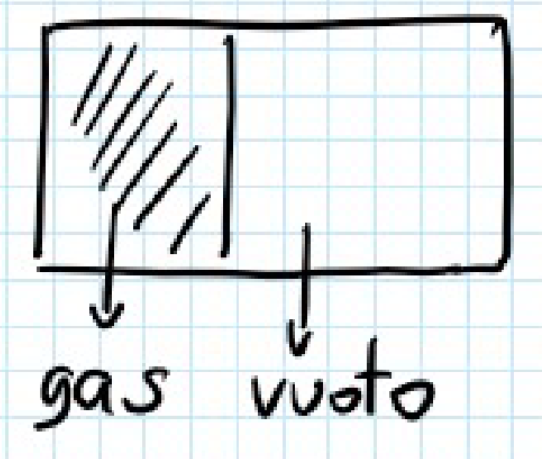
\includegraphics[width=3.3cm]{images/stato_iniziale_espansione_libera_Joule.png}
\end{figure}

\noindent
Consideriamo un contenitore adiabatico separato internamente da una parete adiabatica. In uno dei due volumi si trova un gas ideale, il secondo \`e vuoto.
\smallskip

\noindent
Improvvisamente eliminiamo la parete interna e lasciamo che il gas si espanda\footnote{notiamo che questo NON \`e una processo quasistatico.}.\smallskip

\noindent
Chiaramente $Q=W=0$ in quanto il vuoto non subisce/effettua lavoro e non scambia calore, dunque $\Delta U=0$.\\
Segue che $\mu_J=\ppb VTU=\dd VT$ e Joule ha misurato che in queste circostanze la seconda \`e nulla, dunque
\[0=\ppb VTU\pasgnl={(\ref{ProprietaDerivateParziali})}-\pa{\ppb UVT}\ii\pa{\ppb TUV}\ii=-\ppb VUT\frac1{C_V},\]
in particolare $\displaystyle\ppb VUT=0$.\medskip

\noindent Poich\'e in un gas ideale $p$ \`e determinata da $V$ e $T$, $U=U(V,T)$. Per quanto appena detto $U$ non dipende da $V$, quindi dipende solo da $T$.
\end{proof}


\begin{corollary}
In un gas ideale, a prescindere dal tipo di processo,
\[\boxed{dU=C_V dT}\]
\end{corollary}
\begin{proof}
Ricordiamo che
\[C_V=\ppb TUV,\]
ma poich\'e $U$ non dipende da $V$ possiamo scrivere
\[C_V=\dd TU,\]
che \`e la tesi.
\end{proof}

\begin{proposition}[Relazione di Mayer]\label{RelazioneMayer}
Per gas ideali si ha che $c_p-c_V=R$, o equivalentemente $C_p-C_V=nR$.
\end{proposition}
\begin{proof}
Ricordiamo (\ref{CoefficienteEspansioneECompressibilitaIsotermaPerGasIdeali}) che per gas ideali $\al=T\ii$. Poich\'e $U$ dipende solo da $T$ si ha che
\[0=\ppb VUT\pasgnl={(\ref{DerivataEnergiaInternaRispettoAlVolume})}\frac{C_p-C_V}{V\al}-p,\]
da cui
\[C_p-C_V=pV\al=\frac{nRT}T=nR.\]
\end{proof}

\begin{notation}
Denotiamo il rapporto $\frac{C_V}{C_p}=\frac{c_V}{c_p}$ con $\gamma$.
\end{notation}



\begin{fact}[Calore specifico a volume costante in funzione dei gradi di libert\`a]
In un gas ideale
\[C_V=\frac\nu2nR\]
dove $\nu$ \`e il \textbf{numero di gradi di libert\`a}.
\end{fact}
\begin{remark}
Per un gas ideale monoatomico $\nu=3$, mentre per un gas biatomico $\nu=5$.\\
Segue che
\[c_V^{mono}=\frac32R\approx 12.47\frac{\mathrm{J}}{\mathrm{K\ mol}},\qquad c_V^{bi}=\frac52R\approx 20.74\frac{\mathrm{J}}{\mathrm{K\ mol}}.\]
Da queste scritture segue anche che
\[c_p^{mono}=\frac52R,\quad \gamma^{mono}=\frac53,\quad\qquad c_p^{bi}=\frac72R,\quad \gamma^{bi}=\frac75.\]
\end{remark}

\begin{remark}[L'aria \`e un gas ideale biatomico]
L'aria \`e composta principalmente da particelle biatomiche ($O_2$ e $N_2$).
\end{remark}

\begin{proposition}[Calore infinitesimale con capacit\`a]\label{CaloreInfinitesimaleConCapacita}
Per gas ideali valgono le seguenti equazioni
\begin{enumerate}
\item $\delta Q=C_VdT+pdV$
\item $\delta Q=C_p dT-Vdp$.
\end{enumerate}
\end{proposition}
\begin{proof}
Mostriamo i due punti:
\setlength{\leftmargini}{0cm}
\begin{itemize}
\item[$\boxed{1}$] Ricordiamo la relazione \[\delta Q=\under{=C_V}{\ppb TUV} dT+\pa{{\ppb VUT}+p}dV,\]
da cui, usando il fatto che $\ppb VUT=0$, troviamo che $\delta Q=C_V dT+pdV$.
\item[$\boxed{2}$] Osserviamo che il differenziale di $pV=nRT$ \`e
\[nRdT=pdV+Vdp,\]
da cui sfruttando la relazione precedente
\[\delta Q=C_VdT+pdV=({C_V+nR})dT-Vdp\pasgnl={(\ref{RelazioneMayer})}C_p dT-Vdp.\]
\end{itemize}
\setlength{\leftmargini}{0.5cm}
\end{proof}
\begin{remark}
Osservando la prima equazione ricaviamo nuovamente che $\delta Q$ non \`e un differenziale, infatti se lo fosse avremmo il seguente assurdo:
\[0=\ppb V{C_V}T=\ppb TpV=\frac{nR}V\neq 0.\]
\end{remark}


\section{Energia interna, lavoro e calore}

\noindent In questa sezione calcoliamo lavoro, calore e variazione di energia interna per i tipi principali di processi quasistatici.\medskip

\noindent Notiamo che $\Delta U=nc_V\Delta T$ in ogni circostanza in quanto $U$ non dipende da $V$.
\subsection{Isobara}
\begin{proposition}[Energie per isobara]\label{EnergieIsobara}
Per una trasformazione isobara valgono le seguenti identit\`a:
\[W=-nR\Delta T,\quad
Q=nc_p\Delta T,\quad
\Delta U=nc_V\Delta T.\]
\end{proposition}
\begin{proof}
Calcoliamo:
\begin{align*}
W=&-\int_{V_i}^{V_f}pdV\pasgnl={isobara}-p\Delta V\pasgnl={gas ideale}-nR\Delta T\\
Q\pasgnl={isobara}&\int_{T_i}^{T_f}nc_pdT=nc_p\Delta T\\
\Delta U=&Q+W=n(c_p-R)\Delta T=nc_V\Delta T.
\end{align*}
\end{proof}

\subsection{Isocora}
\begin{proposition}[Energie per isocora]\label{EnergieIsocora}
Per una trasformazione isocora valgono le seguenti identit\`a:
\[W=0,\quad
Q=nc_v\Delta T,\quad
\Delta U=nc_V\Delta T.\]
\end{proposition}
\begin{proof}
Calcoliamo:
\begin{align*}
W=&-\int_{V_i}^{V_f}pdV\pasgnlmath={V_i=V_f}0\\
Q\pasgnl={isocora}&\int_{T_i}^{T_f}nc_VdT=nc_V\Delta T\\
\Delta U=&Q+W=nc_V\Delta T.
\end{align*}
\end{proof}

\subsection{Isoterma}
\begin{proposition}[Energie per isoterma]\label{EnergieIsoterma}
Per una trasformazione isoterma valgono le seguenti identit\`a:
\[W=-nRT\log\pa{\frac{V_f}{V_i}},\quad
Q=nRT\log\pa{\frac{V_f}{V_i}},\quad
\Delta U=0.\]
\end{proposition}
\begin{proof}
Poich\'e stiamo considerando un gas ideale \[\Delta U=nc_V\Delta T\pasgnl={isoterma}0.\] 
Per il primo principio si ha $Q=-W$, quindi per concludere basta calcolare il lavoro.
\[W=-\int_{V_i}^{V_f}pdV\pasgnl={gas ideale}-nRT\int_{V_i}^{V_f}\frac1VdV=-nRT\log\pa{\frac{V_f}{V_i}}.\]
\end{proof}

\subsection{Adiabatica}
\begin{proposition}[Equazione di stato per adiabatica]\label{EquazioneStatoAdiabatica}
Poniamo $\gamma=c_p/c_V$. Si ha che $pV^\gamma$ \`e costante seguendo un processo adiabatico.
\end{proposition}
\begin{proof}
Poich\'e il sistema in esame \`e un gas ideale valgono le seguenti uguaglianze
\[0\pasgnl={adiabatica}\delta Q=dU-\delta W\pasgnl={gas ideale}nc_VdT+pdV=\frac{nc_V}{nR}d(pV)+p dV.\]
Segue che
\[-\frac{c_VV}{\cancel{R}}dp=\pa{\frac{pc_V+pR}{\cancel{R}}}dV\pasgnl={(\ref{RelazioneMayer})}\frac{pc_p}{\cancel{R}}dV,\]
da cui
\[-\frac{dp}p=\gamma\frac{dV}V.\]
Integrando troviamo
\[-\log p+Const.=\gamma\log V\coimplies \log pV^\gamma=Const.\coimplies pV^\gamma=e^{Const.}\]
che \`e quello che volevamo mostrare.
\end{proof}
\begin{remark}
Si ha che \[c_v=\frac R{\gamma-1}.\]
\end{remark}
\begin{proof}
Per definizione di $\gamma$
\[c_v=\frac{c_p}\gamma\pasgnl={(\ref{RelazioneMayer})}\frac{R+c_v}\gamma,\]
dunque
\[\gamma c_v=c_v+R\]
e la tesi segue.
\end{proof}

\begin{proposition}[Energie per adiabatica]\label{EnergieAdiabatica}
Per una trasformazione adiabatica valgono le seguenti identit\`a:
\[W=\frac{p_fV_f-p_iV_i}{\gamma-1},\quad
Q=0,\quad
\Delta U=\frac{p_fV_f-p_iV_i}{\gamma-1}.\]
\end{proposition}
\begin{proof}
Poich\'e il processo \`e adiabatico, $Q=0$. Segue per il primo principio che $\Delta U=W$. Dato che stiamo considerando un gas ideale
\[\Delta U=nc_V\Delta T=n\frac R{\gamma-1}\Delta T=\frac 1{\gamma-1}\Delta (pV)=\frac{p_fV_f-p_iV_i}{\gamma-1}.\]
\end{proof}

\begin{remark}
Potevamo ricavare energia e lavoro anche sfruttando la relazione \[pV^\gamma=p_iV_i^\gamma=p_fV_f^\gamma,\] ma avendola ricavata come sopra sappiamo che l'espressione \`e \textbf{valida anche per processi adiabatici NON quasistatici}.
\end{remark}

\section{Ciclo di Carnot per Gas ideali}

\begin{proposition}[Efficienza del ciclo di Carnot]\label{EfficienzaCicloCarnot}
L'efficienza di un ciclo di Carnot per gas ideali tra le temperature $T_H$ e $T_L$ \`e data da
\[\eta=1-\frac{T_L}{T_H}.\]
\end{proposition}
\begin{proof}
Calcoliamo che quantit\`a coinvolte:
\[\abs{Q_H}=Q_{AB}\pasgnl={isoterma.}-W_{AB}=\int_A^BpdV=nRT_H\log\pa{\frac{V_B}{V_A}}>0\]
\[\abs{Q_L}=-Q_{CD}\pasgnl={isoterma.}W_{CD}=-\int_C^DpdV=nRT_L\log\pa{\frac{V_C}{V_D}},\]
\[\eta=1-\frac{\abs{Q_L}}{\abs{Q_H}}=1-\frac{T_L\log(V_C/V_D)}{T_H\log(V_B/V_A)}=1-\frac{T_L}{T_H},\]
dove nell'ultimo conto abbiamo usato le equazioni per le adiabatiche:
\[\pa{\frac{V_B}{V_C}}^{\gamma-1}=\frac{T_L}{T_H},\quad \pa{\frac{V_D}{V_A}}^{\gamma-1}=\frac{T_H}{T_L}\implies \frac{V_B}{V_A}=\frac{V_C}{V_D}.\]
\end{proof}

\begin{remark}[Efficienza massima]
Poich\'e il ciclo di Carnot \`e reversibile, per il teorema di Carnot (\ref{TeoremaDiCarnot}) il valore
\[1-\frac{T_L}{T_H}\]
\`e la massima efficienza possibile per un qualsiasi ciclo reversibile che agisce tra due sorgenti alle tempersture indicate.
\end{remark}

\begin{remark}[Coefficiente di prestazione massimo per gas ideale]
Per quanto detto il coefficente di prestazione massimo \`e
\[\frac{1-\eta_{Carnot}}{\eta_{Carnot}}= \frac{T_L}{T_H-T_L}.\]
Se $T_L=4^\circ\mathrm{C}$ e $T_H=20^\circ\mathrm{C}$ (caso tipico del frigorifero casalingo) allora $COP_{max}\approx 17.3$. Tipicamente $COP\approx 4$.
\end{remark}
\begin{remark}[Massima efficienza di una pompa di calore realizzata con gas ideale]
Per una pompa di calore, la massima efficienza \`e data da
\[\frac{T_H}{T_H-T_L}.\]
\end{remark}


\section{Potenziali termodinamici}
Il calore scambiato per trasformazioni reversibili nei gas ideali si pu\`o sviluppare in
\[\rbar{\delta Q}_{rev}=dU+pdV=C_VdT+\frac{nRT}VdV,\]
da cui
\[dS=\frac{\delta Q}T=\frac{C_V}TdT+\frac{nR}VdV.\]
\begin{proposition}[Entropia per gas ideali]\label{EntropiaGasIdeali}
Valgono le seguenti espressioni:
\begin{align*}
S_B-S_A=&C_V\log\pa{\frac{T_B}{T_A}}+nR\log\pa{\frac{V_B}{V_A}}\\
=&C_V\log\pa{\frac{p_BV_B^\gamma}{p_AV_A^\gamma}}\\
=&nc_p\log\pa{\frac{T_B}{T_A}}-nR\log\pa{\frac{p_B}{p_A}}
\end{align*}
\end{proposition}
\begin{proof}
Ricaviamo le tre formulazioni:
\begin{itemize}
\item Integrando $dS=\frac{C_V}TdT+\frac{nR}VdV$ troviamo la prima espressione.
\item Sfruttando la proporzionalit\`a $\displaystyle \frac{T_B}{T_A}=\frac{p_BV_B}{p_AV_A}$ possiamo rielaborare la prima forma come segue
\begin{align*}
S_B-S_A=&C_V\log\pa{\frac{p_B}{p_A}}+(C_V+nR)\log\pa{\frac{V_B}{V_A}}=\\
=&C_V\log\pa{\frac{p_B}{p_A}}+C_p\log\pa{\frac{V_B}{V_A}}=\\
=&C_V\pa{\log\pa{\frac{p_B}{p_A}}+\log\pa{\pa{\frac{V_B}{V_A}}^\gamma}}=\\
=&C_V\log\pa{\frac{p_BV_B^\gamma}{p_AV_A^\gamma}},
\end{align*}
ricavando la seconda espressione.
\item Ricordiamo che $\delta Q=nc_p dT-Vdp$. Dividendo per $T$ e poi integrando\footnote{stiamo usando che $-V/T=-nR/p$.} ricaviamo
\[S_B-S_A=nc_p\log\pa{\frac{T_B}{T_A}}-nR\log\pa{\frac{p_B}{p_A}}.\]
\end{itemize}
\end{proof}


\begin{remark}
Se ci spostiamo lungo una adiabatica reversibile, dalla seconda formula ricaviamo $\Delta S=0$ come ci aspettiamo.
\end{remark}

\begin{proposition}[Entropia in gas ideali per processi standard]
Valgono le seguenti espressioni:

\begin{itemize}
\item[$\boxed{\text{Isocora}}$] $\Delta S=nc_V\log\pa{\frac{T_B}{T_A}}\leadsto dS=nc_V\frac{dT}T,$
\item[$\boxed{\text{Isobara}}$] $\Delta S=nc_p\log\pa{\frac{T_B}{T_A}}\leadsto dS=nc_p\frac{dT}T.$
\item[$\boxed{\text{Isoterma}}$] $\Delta S=nR\log\pa{\frac{V_B}{V_A}}=-nR\log\pa{\frac{p_B}{p_A}}.$
\end{itemize}
\end{proposition}
\begin{proof}
Basta applicare le espressioni trovate (\ref{EntropiaGasIdeali}).
\end{proof}

\begin{remark}
Si ha che
\[dH=dU+pdV+Vdp=C_VdT+d(pV)=n(c_V+R)dT=nc_pdT.\]
\end{remark}

\begin{remark}
Poich\'e nei gas ideali $U$ dipende solo da $T$ e $pV=nRT$, si ha che anche $H$ dipende solo da $T$ per gas ideali. Segue che possiamo testare se un gas \`e ideale verificando se $\mu_{JT}=0$ o meno.
\end{remark}












\section{Equazione di stato dei gas reali}
Cosa pu\`o contribuire a negare l'approssimazione di gas ideale?
\begin{itemize}
\item \textbf{Interazione attrattiva tra particelle:} Una particella vicino al bordo \`e attratta dalle particelle pi\`u interne, dunque la pressione interna al gas \`e pi\`u grande di quella misurata 
\[p_{real}=p+a\frac {n^2}{V^2}.\]
\item \textbf{Volume occupato dalle particelle:} Le particelle in genere occupano un volume
\[V_{real}=V-bn\]
\end{itemize}
\begin{fact}[Legge di Van der Waals]
In prima approssimazione l'equazione di \textbf{Van del Waals}
\[\pa{p+a \frac{n^2}{V^2}}(V-bn)=nRT.\]
\end{fact}
\begin{remark}
Di solito $a$ si aggira tra $10^{-2}$ e $10$ $\displaystyle\frac{\ell^2\mathrm{atm}}{\mathrm{mol}^2}$, mentre $b$ si aggira tra $10^{-2}$ e $10^{-1}$ $\ell/\mathrm{mol}$.
\end{remark}

\noindent
Sotto una temperatura critica, le isoterme secondo l'equazione di Van der Waals diventano cubiche con un picco e una valle, in realt\`a quello che succederebbe nella realt\`a \`e che raggiungiamo le condizioni per \textit{transizioni di fase}.